% Paquets généraux
\documentclass[a4paper,12pt,titlepage,twoside]{article}
\usepackage[T1]{fontenc}
\usepackage[utf8]{inputenc}
\usepackage[french]{babel}
\addto\captionsfrench{%
  \renewcommand{\tablename}{Tableau}%
}
\usepackage[gen]{eurosym}
%\usepackage[dvips]{graphicx}
\usepackage{fancyhdr}
\usepackage{pdfpages} 
\usepackage{multido}
\usepackage{hyperref}
%\usepackage{textcomp}
\usepackage{schemabloc}
\usepackage[bitstream-charter]{mathdesign}
\usepackage{array}
\newcolumntype{P}[1]{>{\centering\arraybackslash}p{#1}}

\newcommand{\id}{54}
\newcommand{\nom}{Liaisons mécaniques}
\newcommand{\sequence}{04}
\newcommand{\num}{01}
\newcommand{\type}{TP}
\newcommand{\descrip}{Modélisation d'un solide. Comportement des liaisons mécaniques. Modéliser les mécanismes du laboratoire par un schéma cinématique, paramétré.}
\newcommand{\competences}{A3-C4: Analyse d'architecture et de comportement \\ &  Mod1-C1: Isolement d'un solide ou d'un système de solides \\ &  Mod2-C10-1: Modèle de solide indéformable \\ &  Mod2-C11: Modélisation géométrique et cinématique des mouvements entre solides indéformables \\ &  Mod2-C12: Modélisation cinématique des liaisons entre solides \\ &  Mod2-C15: Modélisation des actions mécaniques \\ &  Rés-C6: Utilisation d'un solveur ou d'un logiciel multi physique \\ &  Com1-C1: Différents descripteurs introduits dans le programme \\ &  Com2-C4: Outils de communication}
\newcommand{\nbcomp}{9}
\newcommand{\systemes}{Plateforme Stewart}
\newcommand{\systemessansaccent}{Plateforme Stewart}
\newcommand{\ilot}{2}
\newcommand{\ilotstr}{02}
\newcommand{\dossierilot}{\detokenize{Ilot_02 Plateforme Stewart}}
\newcommand{\imageun}{Plateforme}

\newcommand{\urlsysteme}{\href{https://www.costadoat.fr/systeme/57}{Ressources système}}
\newcommand{\matlabsimscape}{\href{https://github.com/Costadoat/Sciences-Ingenieur/raw/master/Systemes/Plateforme Stewart/Plateforme_Stewart_Simscape.zip}{Modèle Simscape}}
\newcommand{\solidworks}{\href{https://github.com/Costadoat/Sciences-Ingenieur/raw/master/Systemes/Plateforme Stewart/Plateforme_Stewart_Solidworks.zip}{Modèle Solidworks}}
\newcommand{\edrawings}{\href{https://github.com/Costadoat/Sciences-Ingenieur/raw/master/Systemes/Plateforme Stewart/Plateforme_Stewart.EASM}{Modèle eDrawings}}
\newcommand{\test}{Stewart_param1}
\newcommand{\testi}{Stewart_param2}
\newcommand{\testii}{Stewart_param3}
\newcommand{\testiii}{Stewart_param4}
\newcommand{\testiiii}{Stewart_euler}

\newcommand{\institute}{Lycée Dorian}

\usepackage{fancyvrb}
\usepackage{color}
\usepackage{xcolor}
\usepackage{colortbl}
\usepackage{helvet}
\renewcommand{\familydefault}{\sfdefault}
\usepackage{amsfonts}
\usepackage{amsmath}
%\usepackage{xspace}
\usepackage{varioref}
\usepackage{tabularx}
%\usepackage{floatflt}
\usepackage{graphics}
\usepackage{wrapfig}
\usepackage{textcomp}
\usepackage{tikz}
\usepackage{wrapfig}
\usepackage{gensymb}
\usepackage[percent]{overpic}
\usepackage[european]{circuitikz}
\usetikzlibrary{babel}
\usepackage{ifthen}
\usepackage{cancel}
\usepackage{etoolbox}
\usepackage{multirow}
%\usepackage{boxedminipage}
\definecolor{gris25}{gray}{0.75}
\definecolor{bleu}{RGB}{18,33,98}
\definecolor{bleuf}{RGB}{42,94,171}
\definecolor{bleuc}{RGB}{231,239,247}
\definecolor{rougef}{RGB}{185,18,27}
\definecolor{rougec}{RGB}{255,188,204}%255,230,231
\definecolor{vertf}{RGB}{103,126,82}
\definecolor{vertc}{RGB}{220,255,191}
\definecolor{forestgreen}{rgb}{0.13,0.54,0.13}
\definecolor{blcr}{rgb}{0.59,0.69,0.84}
\definecolor{blfr}{rgb}{0.32,0.51,0.75}
\definecolor{orfr}{rgb}{0.90,0.42,0.15}
\definecolor{orcr}{rgb}{0.90,0.65,0.50}
\definecolor{orangef}{rgb}{0.659,0.269,0.072}
\definecolor{orange}{rgb}{0.58,0.35,0.063}
\definecolor{orangec}{rgb}{0.43,0.32,0.25}
\definecolor{rcorrect}{rgb}{0.6,0,0}
\definecolor{sequence}{rgb}{0.75,0.75,0.75}
\definecolor{competences}{rgb}{0.61,0.73,0.35}
\definecolor{grisf}{HTML}{222222}
\definecolor{grisc}{HTML}{636363}
\definecolor{normal}{HTML}{4087c4}
\definecolor{info}{HTML}{5bc0de}
\definecolor{success}{RGB}{92,184,92}
\definecolor{warning}{RGB}{240,173,78}
\definecolor{danger}{RGB}{217,83,79}
\hypersetup{                    % parametrage des hyperliens
    colorlinks=true,                % colorise les liens
    breaklinks=true,                % permet les retours à la ligne pour les liens trop longs
    urlcolor= blfr,                 % couleur des hyperliens
    linkcolor= orange,                % couleur des liens internes aux documents (index, figures, tableaux, equations,...)
    citecolor= forestgreen                % couleur des liens vers les references bibliographiques
    }

% Mise en page
\pagestyle{fancy}

\setlength{\hoffset}{-18pt}
\setlength{\oddsidemargin}{0pt} 	% Marge gauche sur pages impaire2s
\setlength{\evensidemargin}{0pt} 	% Marge gauche sur pages paires
\setlength{\marginparwidth}{00pt} 	% Largeur de note dans la marge
\setlength{\headwidth}{481pt} 	 	% Largeur de la zone de tête (17cm)
\setlength{\textwidth}{481pt} 	 	% Largeu\textbf{r de la zone de texte (17cm)
\setlength{\voffset}{-18pt} 		% Bon pour DOS
\setlength{\marginparsep}{7pt}	 	% Séparation de la marge
\setlength{\topmargin}{-30pt} 		% Pas de marge en haut
\setlength{\headheight}{55pt} 		% Haut de page
\setlength{\headsep}{20pt} 		% Entre le haut de page et le texte
\setlength{\footskip}{30pt} 		% Bas de\textbf{ page + séparation
\setlength{\textheight}{700pt} 		% Hauteur de l'icone zone de texte (25cm)
\setlength\fboxrule{1 pt}
\renewcommand{\baselinestretch}{1}
\setcounter{tocdepth}{1}
\newcommand{\cadre}[2]
{\fbox{
  \begin{minipage}{#1\linewidth}
   \begin{center}
    #2\\
   \end{center}
  \end{minipage}
 }
}

\newcommand{\repon}[1]
{
~\ \\
\begin{tabular}{|m{\linewidth}|}
 \hline
\multido{}{#1}{\\ \hline}
\end{tabular}
}

\newcounter{num_quest} \setcounter{num_quest}{0}
\newcounter{num_rep} \setcounter{num_rep}{0}
\newcounter{num_cor} \setcounter{num_cor}{0}

\newcommand{\question}[1]{\refstepcounter{num_quest}\par
~\ \\ \parbox[t][][t]{0.15\linewidth}{\textbf{Question \arabic{num_quest}}}\parbox[t][][t]{0.85\linewidth}{#1}\par
}


\newcommand{\reponse}[3]
{\refstepcounter{num_rep}
\noindent
\rule{\linewidth}{.5pt}\\
\textbf{Question \arabic{num_rep}:} ~\ \\
\ifdef{\public}{\multido{\i=1+1}{#1}{~\ \\}#2}{#3}
}

\newcommand{\cor}
{\refstepcounter{num_cor}
\noindent
\rule{\linewidth}{.5pt}
\textbf{Question \arabic{num_cor}:} \\
}

\newcommand{\repcarre}[2]
{
~\ \\
\begin{tikzpicture}
\draw [fill=white] (0,0) rectangle +(\linewidth,#1);
\node[align=left] at (1.1,#2-0.3) {\textbf{Question #1:}};
\end{tikzpicture}
}

\newcommand{\titre}[1]
{\begin{center}
\cadre{0.8}{\huge #1} 
\end{center}
}


% En tête et pied de page
\lhead{\nom}
\rhead{
\includegraphics[width=2cm]{../../img/logo}}
\lfoot{\auteurun,\ \auteurdeux}
\cfoot{Page \thepage}

\fancypagestyle{documentreponse}{%
  \fancyhf{}
  \fancyhead[LO]{Nom: ........................ Prénom: ........................}
  \fancyhead[LE]{\nom}
  \fancyhead[RE,RO]{
\includegraphics[width=2cm]{../../img/logo}}
  \lfoot{Document réponse}
  \cfoot{Page \thepage}
   }
  
\fancypagestyle{correction}{%
  \fancyhf{}
  \lhead{\colorbox{danger}{\begin{minipage}{0.65\paperwidth} \textcolor{white}{\textbf{Correction}} \end{minipage}} }
  \rhead{
\includegraphics[width=2cm]{../../img/logo}}
  \lfoot{Renaud Costadoat, Françoise Puig}
  \rfoot{\colorbox{danger}{\begin{minipage}{0.5\paperwidth} \begin{flushright}\textcolor{white}{\textbf{Correction}}\end{flushright} \end{minipage}} }}

\fancypagestyle{correctioninfo}{%
  \fancyhf{}
  \lhead{\colorbox{danger}{\begin{minipage}{0.65\paperwidth} \textcolor{white}{\textbf{Correction}} \end{minipage}} }
  \rhead{
\includegraphics[width=2cm]{../../img/logo}}
  \lfoot{Renaud Costadoat, Juliette Genzmer, Willie Robert}
  \rfoot{\colorbox{danger}{\begin{minipage}{0.6\paperwidth} \begin{flushright}\textcolor{white}{\textbf{Correction}}\end{flushright} \end{minipage}} }}

\renewcommand{\footrulewidth}{0.4pt}

\usepackage{eso-pic}
\newcommand{\BackgroundPic}{%
\put(0,0){%
\parbox[b][\paperheight]{\paperwidth}{%
\vfill
\begin{center}
\hspace{0.5cm}\vspace{0.5cm}
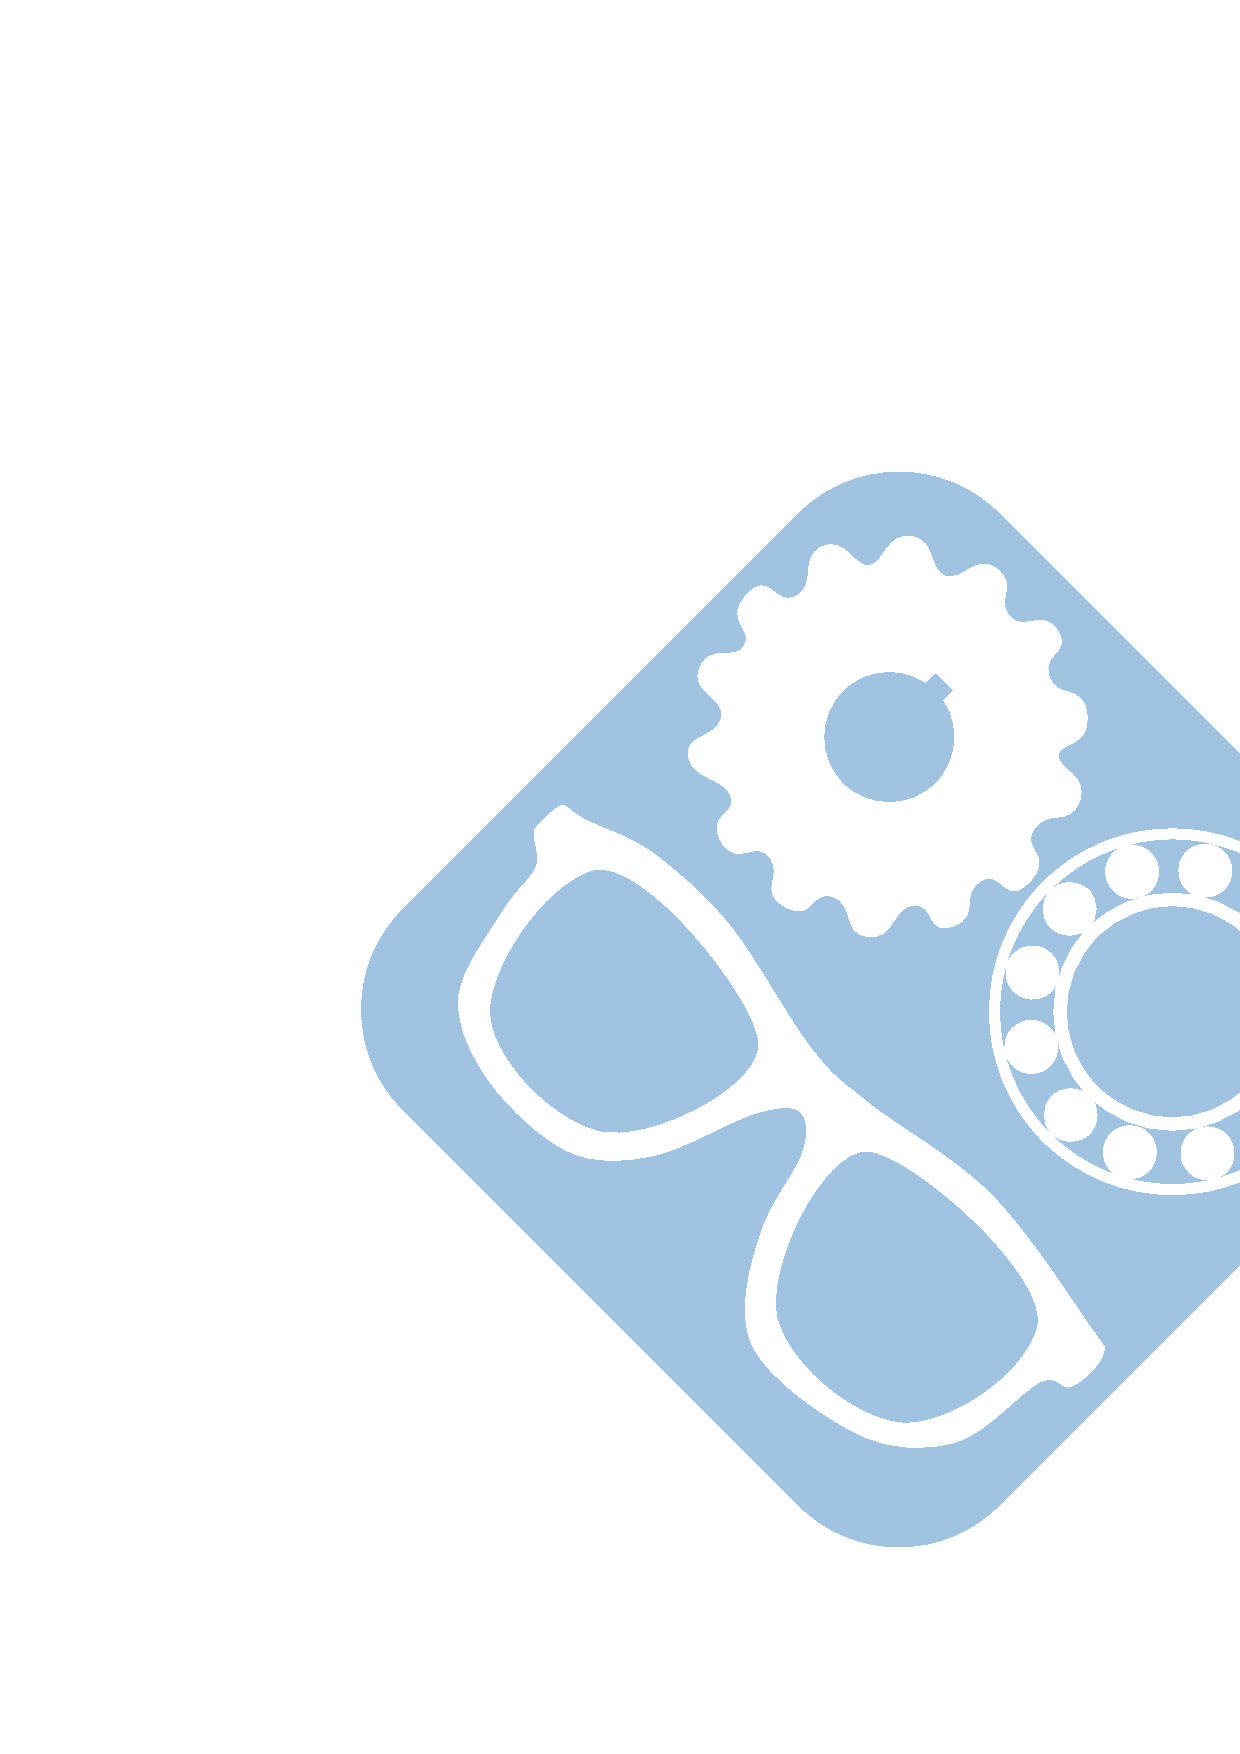
\includegraphics[width=\paperwidth,height=\paperheight,%
keepaspectratio]{../../img/fond3}%
\end{center}
\vfill
}}}

\newcommand{\BackgroundPicdeux}{%
\put(25,-30){%
\parbox[b][\paperheight]{\paperwidth}{%
\vfill
\begin{center}
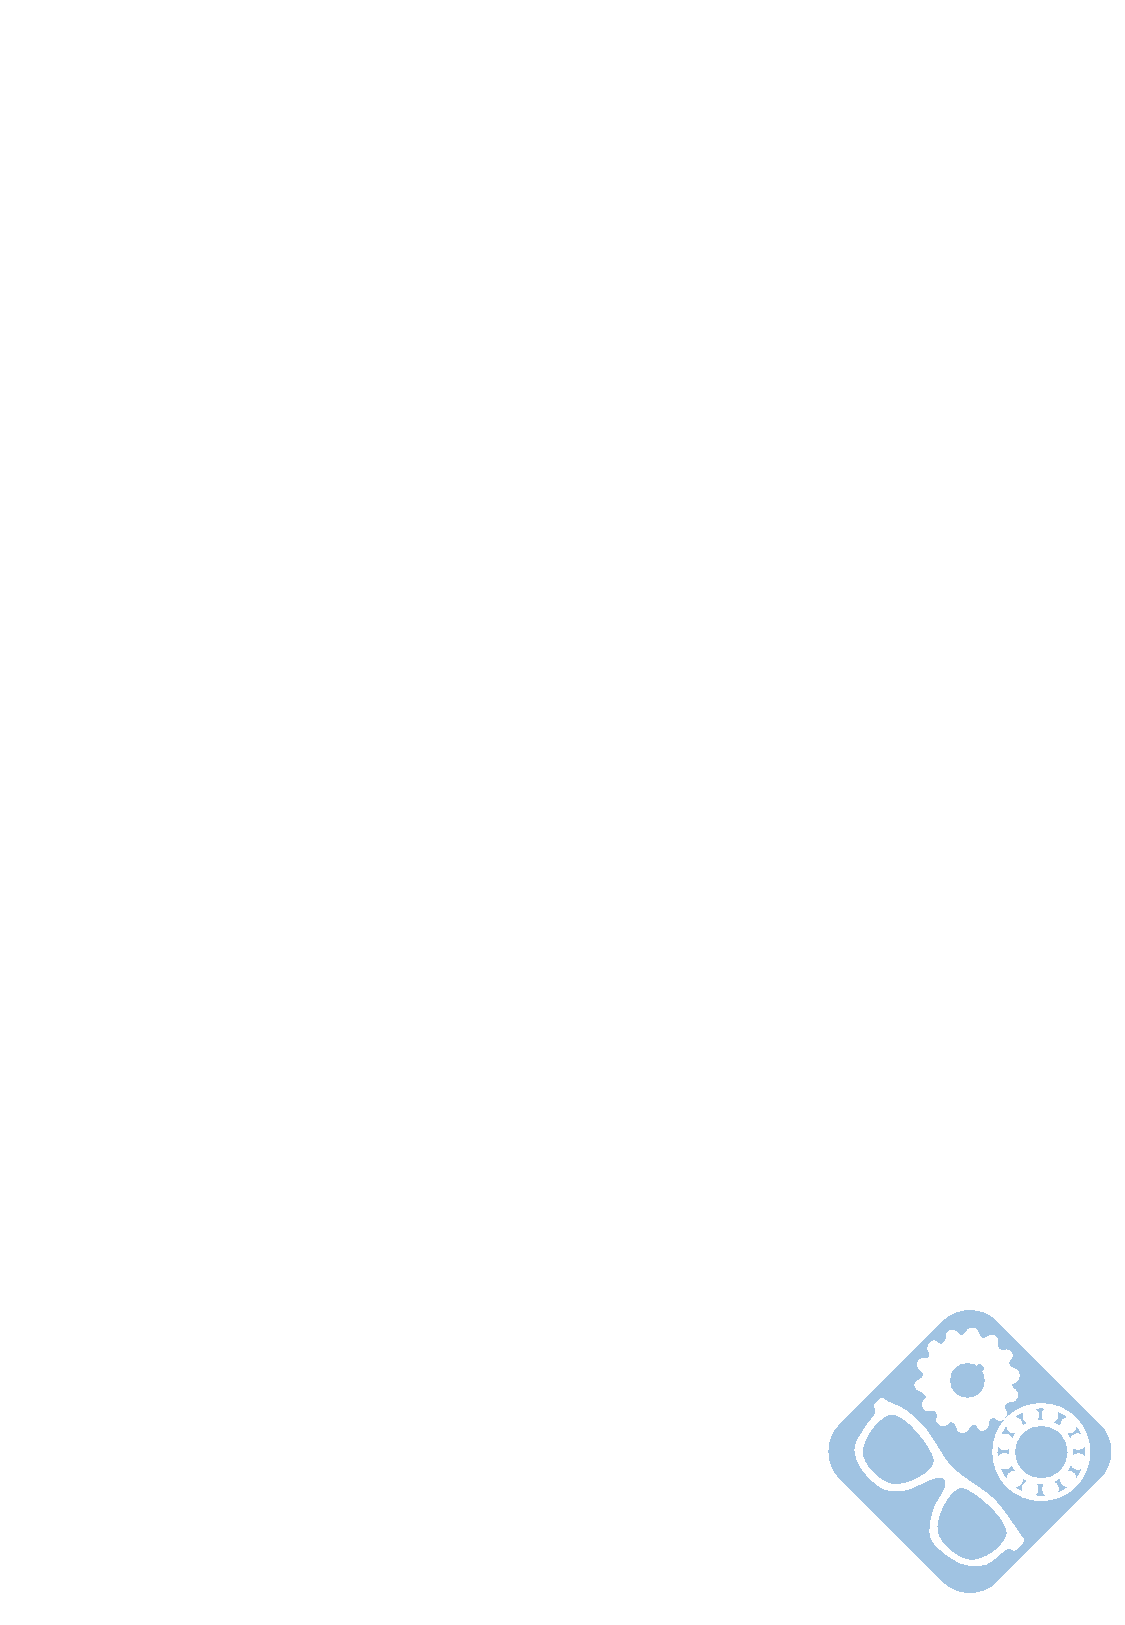
\includegraphics[width=\paperwidth,height=\paperheight,%
keepaspectratio]{../../img/fond4}%
\end{center}
\vfill
}}}

\begin{document}

\pagestyle{empty}

\AddToShipoutPicture*{\BackgroundPic}


\includegraphics[width=2cm]{../../img/logo}

\Huge{DS \num\ - \sujet}

\vspace{1cm}

\ifdef{\prive}{\begin{center}\colorbox{danger}{\Huge{Avec Correction}}\end{center}}{}

\begin{center}
\centering\huge{PTSI}
\end{center}

\vspace{2cm}


\begin{center}
\centering\Large{\jour}
\end{center}

\vspace{2cm}

\normalsize

\tableofcontents

\newpage

\AddToShipoutPicture{\BackgroundPicdeux}

\pagestyle{fancy}

\begin{center}
\Huge \sujet
\end{center}


\normalsize

\section{Présentation générale (30 min)}

\subsection{Introduction}

La société COPEX, installée à Lanester (56 Morbihan) est spécialisée dans les machines et leurs applications à l'environnement. Elle conçoit et fabrique, en particulier du matériel permettant de compacter des déchets de différentes natures, afin d'éventuellement les retraiter ou de les stocker.

L'étude proposée porte sur une Presse-Cisaille type CVB 1 000 T (Cisaille Verticale à Bac de 1 000 tonnes) (figure 1 document 1) destinée à traiter de la ferraille de toute sorte. En fonction des matériaux récupérés, elle permet le compactage sous forme de paquet ou le cisaillage afin de diminuer les volumes lors du transport avant retraitement ou stockage final.

La machine permet deux processus différents :
\begin{itemize}
 \item La réduction de volume par compactage pour l'obtention de paquet,
 \item La réduction de volume par compactage et cisaillage sous forme de bouts de métal découpés à des longueurs variables de 30 à 95 cm.
\end{itemize}

Vue schématique de la machine, de ses mouvements et des détecteurs associés :

\begin{figure}[!h]
\begin{minipage}[t]{0.49\linewidth}
 \centering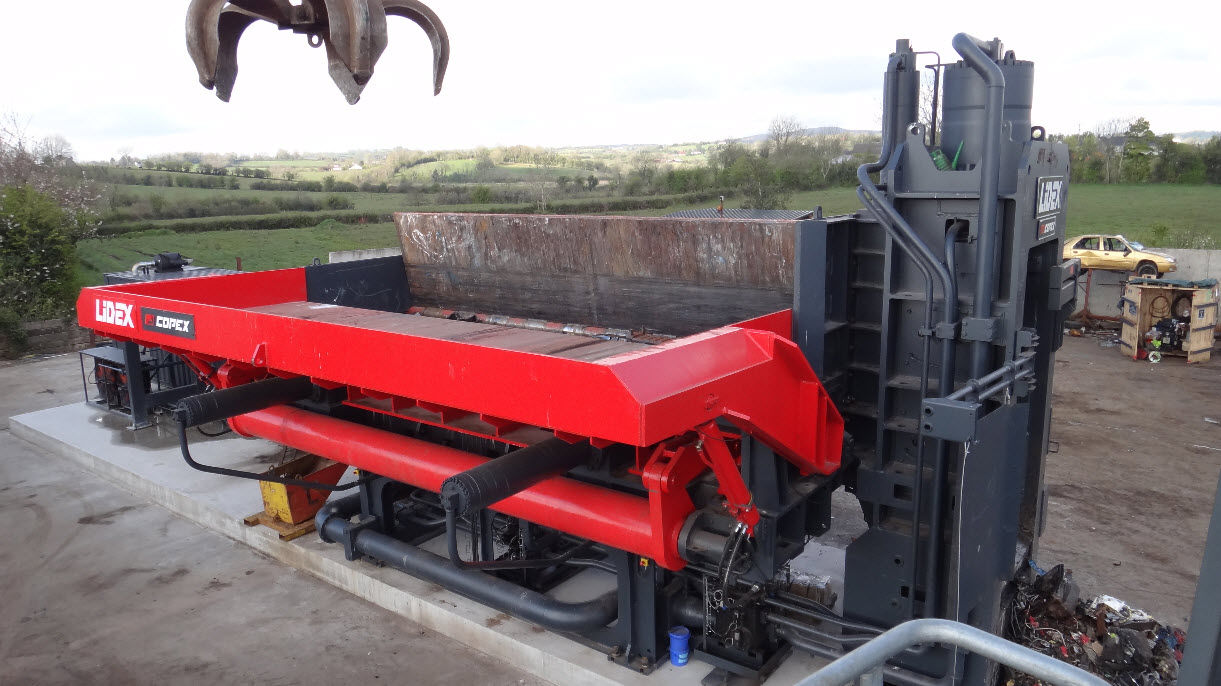
\includegraphics[width=0.9\linewidth]{img/fig1-1}
\end{minipage}\hfill
\begin{minipage}[t]{0.49\linewidth}
 \centering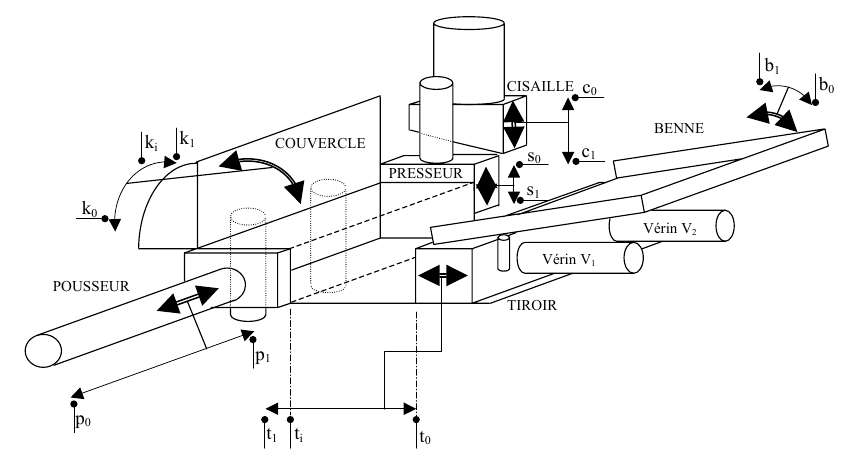
\includegraphics[width=0.9\linewidth]{img/fig1}
\end{minipage}
\end{figure}

\subsection{Cahier des charges du Système}

Voir documents 3 et 4, aux échelles respectives approximatives 1\!:60 et 1\!:30, ainsi que la figure de la page précédente.

Nota : la compréhension très précise du document 3 n'est pas nécessaire. Ce document permet de visualiser les différentes positions relatives des éléments lors du fonctionnement.

La machine est prête pour un chargement et le système est en position initiale :
\begin{itemize}
 \item la \og Cisaille \fg et le \og Presseur \fg sont en position fin de course sortie (position basse), les détecteurs respectifs $c_1$ et $s_1$ sont actionnés,
 \item la \og Benne \fg est en position horizontale au niveau du détecteur $b_0$,
 \item le \og Tiroir \fg est reculé en position fin de course rentrée, le détecteur $t_0$ est actionné,
 \item le \og Couvercle \fg est ouvert en position fin de course, le détecteur $k_0$ est actionné,
 \item le \og Pousseur \fg est reculé en position fin de course, le détecteur $p_0$ est actionné.
\end{itemize}

Le compactage est effectué grâce à quatre actionneurs, pilotés manuellement par l'utilisateur :

\begin{itemize}
 \item Basculement de la \og Benne \fg pour déchargement de la matière dans la caisse de compression,
 \item Retour \og Benne \fg à l'horizontale,
 \item Compression latérale par l'avance partielle du piston \og Tiroir \fg, animé par 2 vérins $V_1$ et $V_2$ jusqu'à l'appui par l'opérateur sur le bouton acquittement,
 \item Recul du \og Tiroir \fg,
 \item Compression supérieure par la fermeture partielle du \og Couvercle \fg, animé par 2 vérins jusqu'à l'appui par l'opérateur sur le bouton acquittement,
 \item Ouverture du \og Couvercle \fg,
 \item Fermeture du \og Couvercle \fg en position horizontale, jusqu'à une position définie par un détecteur de position $k_i$,
 \item Fermeture du \og Tiroir \fg en position coïncidente à la largeur du \og Pousseur \fg, jusqu'à une position définie par un détecteur de position $t_i$,
 \item Compression longitudinale par le piston \og Pousseur \fg, avec un vérin de 120 tonnes (option 320 tonnes). Un détecteur de pression ppm indique à l'opérateur que les ferrailles sont compactées.
\end{itemize}

Le compactage étant terminé, deux modes sont disponibles (document 1, figure 2 et 3) :
\begin{itemize}
 \item Mode \textbf{paquet} qui permet l'évacuation du bloc de métal.
 \item Mode \textbf{cisaille} qui permet le cisaillage et l'évacuation des morceaux de ferraille.
\end{itemize}

\textbf{Mode paquet} (pour le compactage d'un véhicule par exemple).

L'évacuation du paquet est effectuée par un cycle de 2 mouvements successifs en mode automatique :
\begin{itemize}
 \item Montée de la \og Cisaille \fg jusqu'à atteindre le détecteur haut cisaille $c_0$,
 \item Montée de la Porte (\og Presseur \fg) jusqu'à atteindre le détecteur haut presseur $s_0$,
 \item Avance du paquet poussé par le piston \og Pousseur \fg jusqu'à atteindre la fin de course $p_1$.
\end{itemize}

\textbf{Mode cisaille} (pour le cisaillage de matériaux tout venant à dominante métallique).

Le cisaillage des ferrailles est effectué par un cycle de 5 mouvements successifs. Ce cycle se répète $N$ fois en fonction des longueurs $L$ souhaitées par l'opérateur pour les bouts de ferrailles. Le dernier cycle ayant lieu lorsque le fin de course pousseur $p_1$ est atteint.

Chaque cycle est réalisé de la façon suivante :
\begin{itemize}
 \item Montée de la \og Cisaille \fg jusqu'à atteindre le détecteur haut cisaille $c_0$,
 \item Montée de la Porte (\og Presseur \fg) jusqu'à atteindre le détecteur haut presseur $s_0$,
 \item Avance de la matière par le piston \og Pousseur \fg jusqu'à atteindre la position \og poussoir avancé de $L$ \fg, fonction de la longueur des bouts de ferraille souhaitée,
 \item Descente du \og Presseur \fg jusqu'à atteindre une position intermédiaire. Celle-ci permettant d'assurer la pression souhaitée $sp_1$ nécessaire au blocage des ferrailles compactées,
 \item Descente de la \og Cisaille \fg et découpe de la matière jusqu'à atteindre le détecteur bas cisaille $c_1$.
\end{itemize}

En mode \textbf{Paquet} ou mode \textbf{Cisaillage}, lorsque le fin de course pousseur $p_1$ est atteint :
\begin{itemize}
 \item Recul \og Pousseur \fg jusqu'à atteindre fin de course pousseur $p_0$,
 \item Recul du \og Tiroir \fg simultanément à l'ouverture du \og Couvercle \fg jusqu'à atteindre les fins de course respectifs $t_0$ et $k_0$,
 \item Descente \og Cisaille \fg simultanément à la descente du \og Presseur \fg jusqu'à atteindre les positions fins de courses basses $c_1$ et $s_1$	.
\end{itemize}

Nota : Ces cinq mouvements ne peuvent être réalisés simultanément du fait de la limitation des débits du groupe hydraulique.

Une fois l'ensemble des mouvements terminés, la machine est prête pour un nouveau chargement.

\paragraph{Question 1:} Compléter le diagramme de Contexte du système.

\paragraph{Question 2:} Compléter le diagramme des Cas d'Utilisation du système.

\paragraph{Question 3:} Compléter le diagramme de Définition de Blocs.

\paragraph{Question 4:} Sur le diagramme de Blocs Internes, colorier en rouge les flux énergétiques et en bleu les flux de matière.

\section{Étude de l'asservissement du tiroir 1 (1h15)}

Comme nous l'avons étudié précédemment, le déplacement en translation du tiroir $1$ est assuré par deux vérins hydrauliques $V_1$ et $V_2$ nécessitant un palonnier pour éviter l'arc-boutement lors de son déplacement.

Cette étude porte sur une nouvelle solution remplaçant le palonnier par un asservissement en position des deux vérins.

Les deux vérins hydrauliques sont montés en portique en deux points d'ancrage (en parallèle) sur le tiroir. Chaque vérin du type \og mesure en position intégrée \fg (détecteur inductif intégré dans la tige du vérin, résolution $\pm 0,1$ mm) est piloté par un servo-distributeur. Les commandes des deux vérins sont synchronisées pour limiter l'arc-boutement du tiroir (efforts dissymétriques dus à la ferraille à compacter).

On isole l'un des vérins.

Le comportement du vérin peut alors être modélisé à partir du modèle de structure ci-dessous et du paramétrage qui lui est associé.

\begin{figure}[!h]
 \centering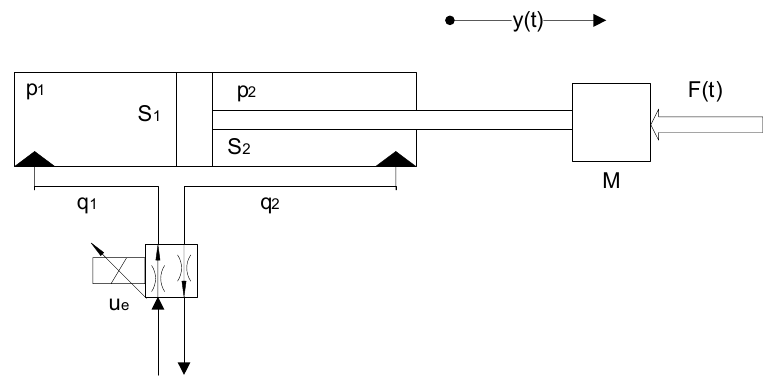
\includegraphics[width=0.7\linewidth]{img/fig3.png}
\end{figure}

On donne :
\begin{itemize}
 \item $M=10^4kg$ : masse de l'équipage mobile ;
 \item $f=3.10^6N.m^{-1}.s$ : la résistance due aux frottements visqueux ;
 \item $K=2,5.10^7N.m^{-1}$ : la raideur hydraulique du vérin ;
 \item $S_1=5.10^{-2}m^2$ : la surface du piston de la chambre d'admission.
\end{itemize}

L'ensemble appelé \og équipage mobile \fg est formé par :
\begin{itemize}
 \item le tiroir,
 \item l'effort variable dû à la ferraille, noté F(t),
 \item la tige du piston du vérin.
\end{itemize}

Sa position notée y(t) est fonction du débit d'huile, noté $q_1(t$), à l'entrée de la chambre d'admission du vérin.

On se place dans l'hypothèse de petit déplacement autour d'un point de fonctionnement (position particulière d'équilibre). Le système peut donc être considéré comme linéaire, continu et invariant.

\subsection{Modélisation de l'équipage mobile}

Après calcul :
\begin{itemize}
 \item L'équation temporelle donnant le déplacement $y_1(t)$ en fonction du débit $q_1(t)$ pour un effort $F(t)$ nul est telle que : 
 $M.\frac{d^2y_1(t)}{dt^2}=K.\int_{0}^{t} \frac{q_1(\tau)}{S_1}d\tau-K.y_1(t)-f.\frac{dy_1(t)}{dt}$
 \item L'équation temporelle donnant le déplacement $y_2(t)$ en fonction de l'effort $F(t)$ pour un débit $q_1(t)$ nul est telle que :
 $M.\frac{d^2y_2(t)}{dt^2}=-K.y_2(t)-f.\frac{dy_2(t)}{dt}+F(t)$
\end{itemize}

\paragraph{Question 5 :} En supposant que les conditions initiales sont nulles, donner dans le domaine de Laplace et sous forme canonique :

\begin{itemize}
 \item La fonction de transfert : $H_1(p)=\frac{Y_1(p)}{Q_1(p)}$ liant le déplacement $y_1(t)$ au débit $q_1(t)$ pour un effort $F(t)$ nul,
 \item La fonction de transfert : $H_2(p)=\frac{Y_2(p)}{F(p)}$ liant le déplacement $y_2(t)$ à l'effort $F(t)$ pour un débit $q_1(t)$ nul.
\end{itemize}
  
\paragraph{Question 6 :} En appliquant le principe de superposition, donner l'équation, dans le domaine de Laplace, liant le déplacement $Y(p)$ au débit $Q_1(p)$ et à l'effort $F(p)$.

\subsection{Modélisation générale du fonctionnement de l'ensemble vérin et distribution}

Pour étudier l'influence du débit, on néglige la contribution de l'effort $F(t)$. La fonction de transfert déplacement-débit est alors :

$G(p)=\frac{Y(p)}{Q_1(p)}=\frac{1}{p.S_1.\left[1+\frac{1}{K}.(f.p+M.p^2)\right]}$

On admettra que ce résultat est généralisable pour toute position de la tige de vérin.

Le servodistributeur proportionnel délivre un débit d'huile $q_1(t)$ proportionnel à sa tension de commande $u_e(t)$ tel que : $q_1(t)=K_e.u_e(t)$, avec $K_e=2.10^{-4}m^3.s^{-1}.V^{-1}$.

Le détecteur de position délivre une tension $u_s(t)$ proportionnelle à la position $y(t)$ du tiroir telle que : $u_s(t)=K_c.y(t)$, avec $K_c=10^3V.m^{-1}$.

\paragraph{Question 7 :} Déterminer les fonctions de transfert $\frac{Q_1(p)}{U_e(p)}$ et $\frac{U_s(p)}{Y(p)}$.

\paragraph{Question 8 :} En déduire la fonction de transfert, dite \og en boucle ouverte \fg, du système tiroir-vérin-distribution dont la transmitance est : $\frac{U_s(p)}{U_e(p)}$

\paragraph{Question 9 :} Déterminer la classe, l'ordre et les caractéristiques de la fonction de transfert ainsi obtenue.

~\

Pour boucler le système :
\begin{itemize}
 \item le signal de la commande du distributeur proportionnel $u_e(t)$ est élaboré à partir :
 \begin{itemize}
  \item d'un élément permettant de comparer $u_s(t)$ à la tension de consigne $u_c(t)$,
  \item d'un amplificateur de gain A.
 \end{itemize}
 \item le signal de tension de consigne est élaboré à partir de la consigne de position y c(t) et d'un potentiomètre modélisable par un gain pur identique à $K_c$.%
\end{itemize}

Ainsi, $u_e(t)=A\times \left[y_c(t)\times K_c - u_s(t)\right]$.


\paragraph{Question 10 :} Calculer la fonction de transfert en boucle fermée : $\frac{Y(p)}{Y_c(p)}$ en fonction des différents coefficients littéraux caractérisant le système.

L'influence de la masse sur le système n'étant pas très importante, elle sera dans la suite négligée.

\paragraph{Question 11:} Donner la nouvelle forme de la fonction de transfert. Déterminer les valeurs caractéristiques de cette fonction de transfert et faire l'application numérique en prenant $A=1$.

~\

La figure donnée sur le document réponse présente le tracé de la réponse de cette fonction de transfert en prenant en entrée un échelon $y_c(t)=1$.

\paragraph{Question 12:} Déterminer littéralement la valeur du dépassement $D\%$, vérifier cette valeur sur la courbe. Déterminer sur la courbe, la valeur du temps de réponse $t_{R,5\%}$.

\section{Analyse d'un mécanisme (45min)}

Le système suivant permet de fermer une vanne.

\begin{center}
 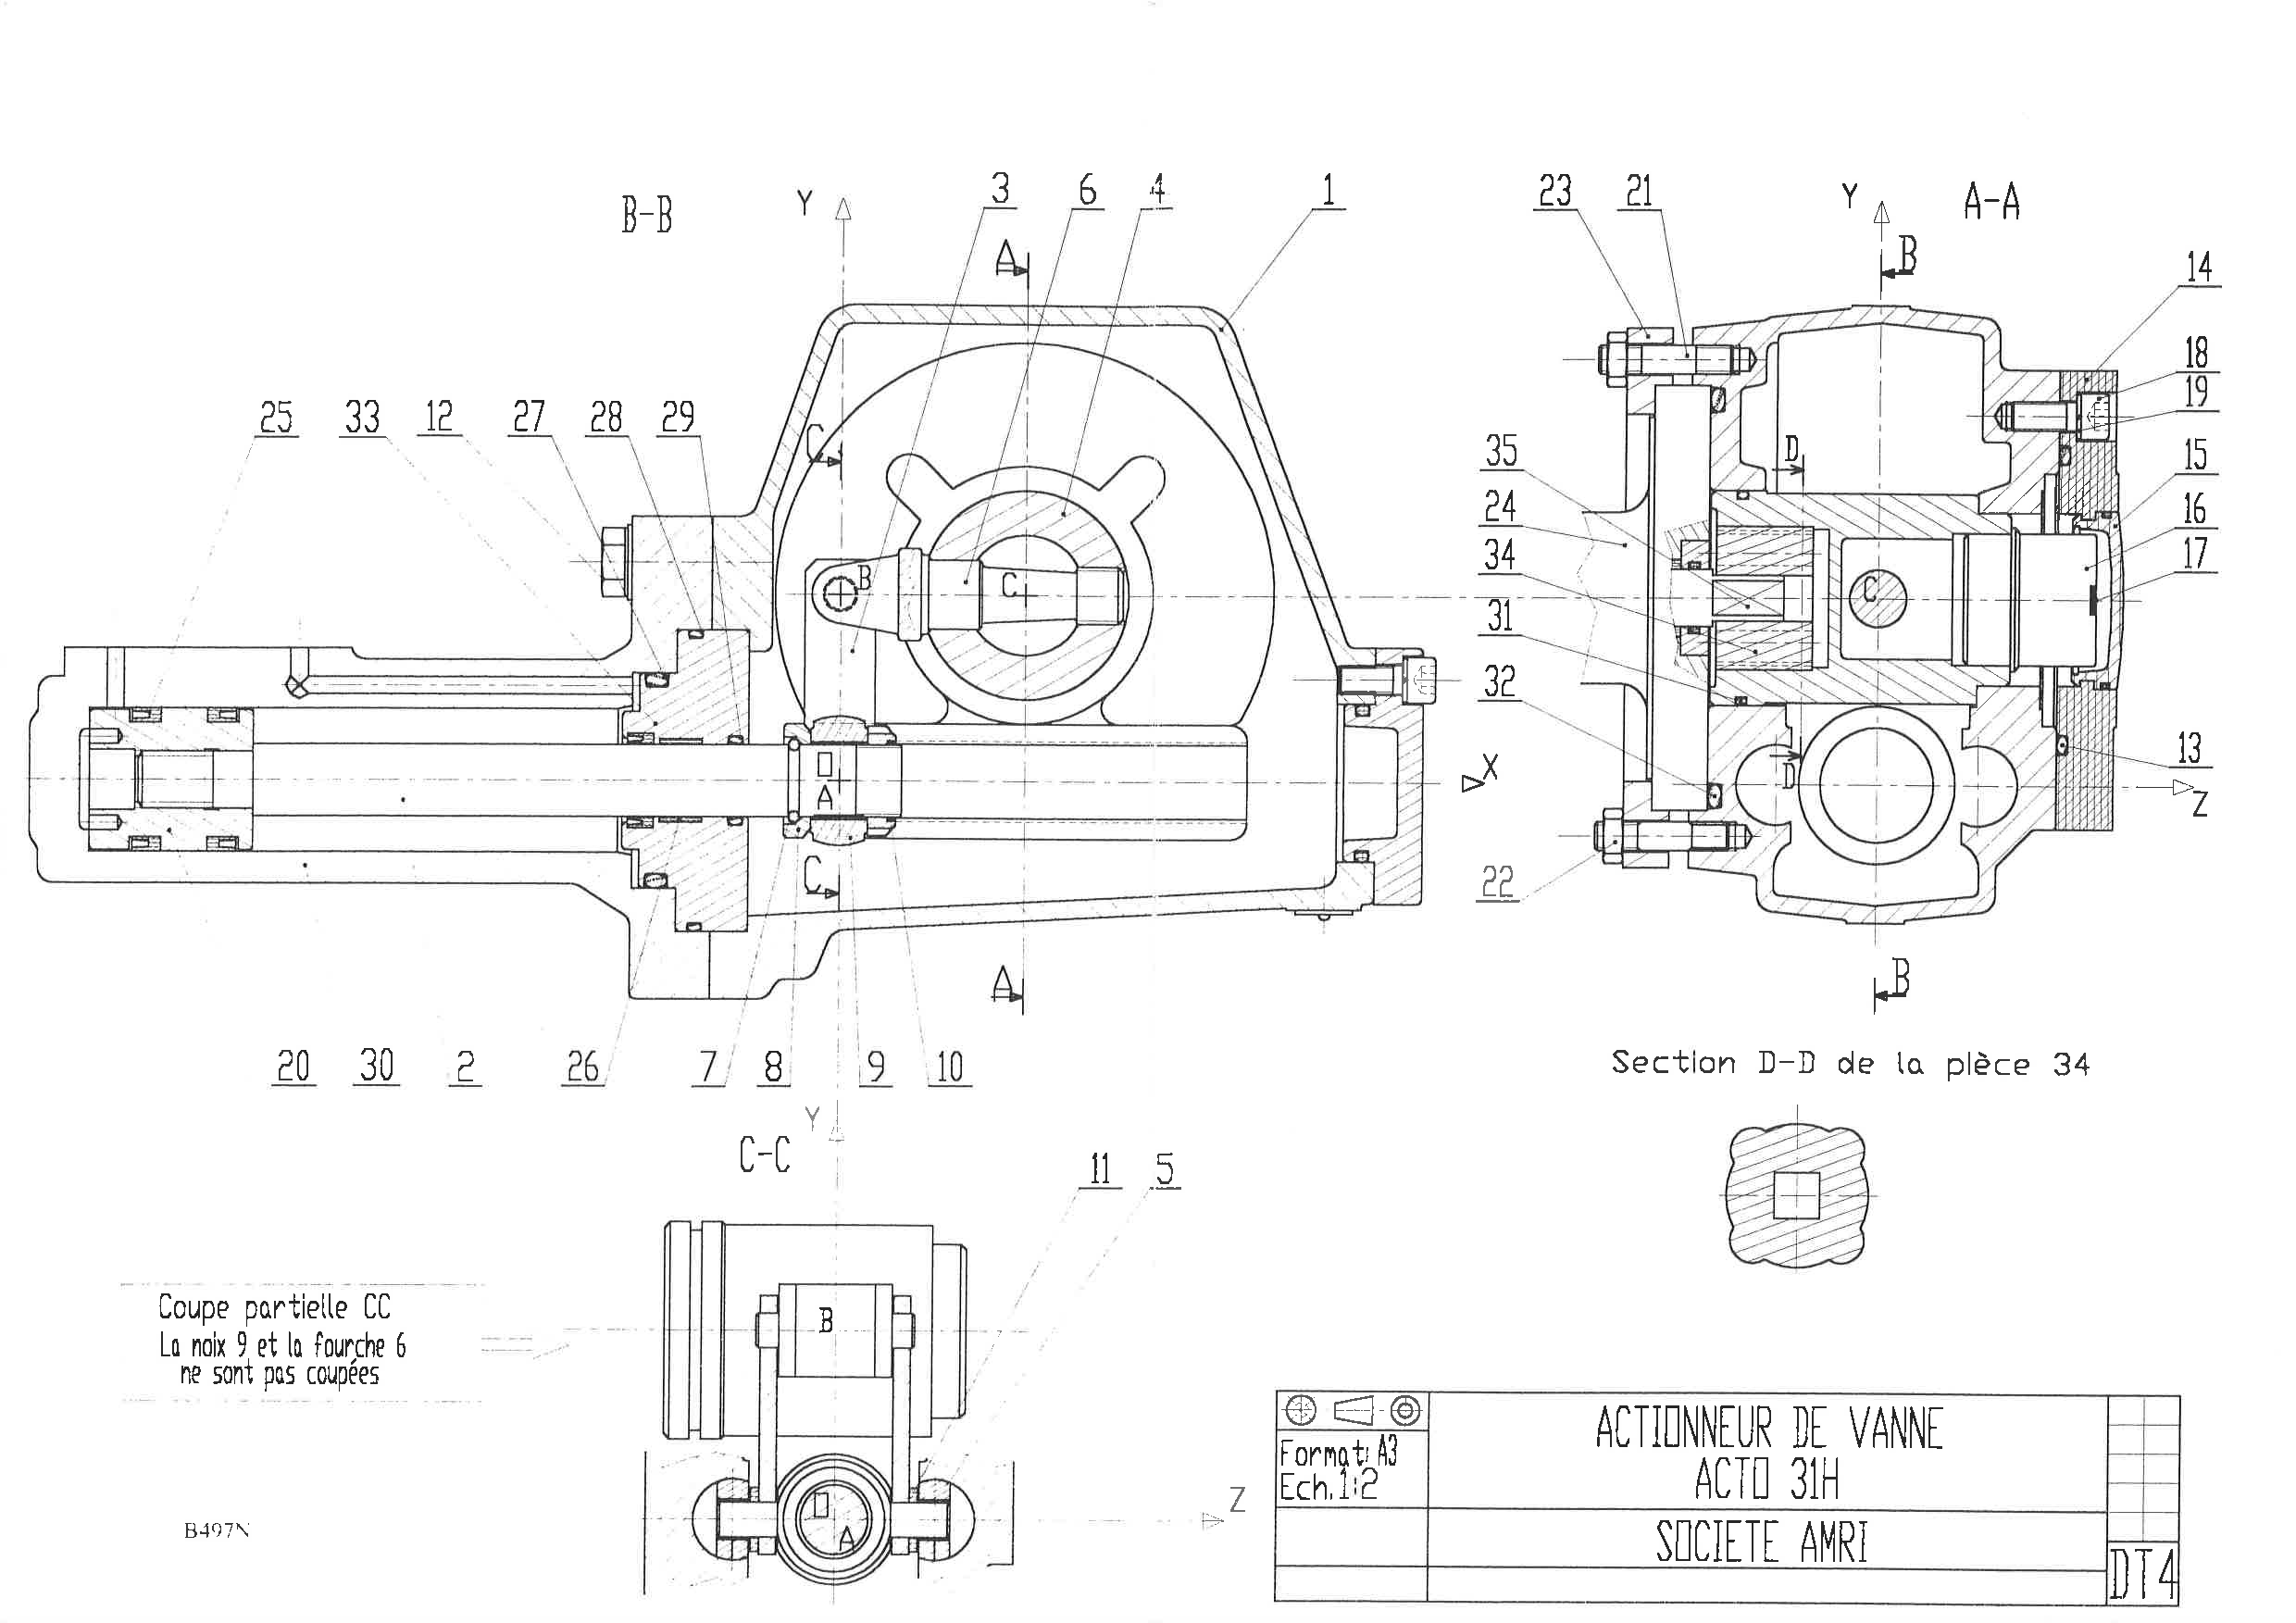
\includegraphics[width=0.8\linewidth]{img/Actionneur_vanne}
\end{center}

\paragraph{Question 13:} Colorier sur le document réponse les classes d'équivalence.

\paragraph{Question 14:} Déterminer quel type d'énergie permet de mettre en mouvement le système de fermeture de la vanne.

\paragraph{Question 15:} Déterminer la longueur du déplacement A, nécessaire à la fermeture de la vanne (rotation de 90\textdegree). Les construction nécessaires seront à effectuer sur le document réponse.

\begin{center}
FIN DU SUJET
\end{center}

\newpage
\cleardoublepage

\section{Documents réponse}

Nom:.....................\\
Prénom:......................

\paragraph{Question 1:}

\begin{center}
 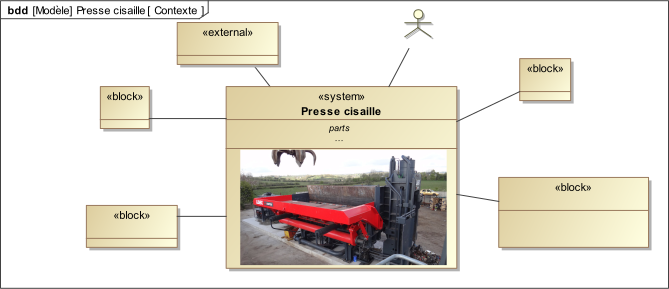
\includegraphics[width=0.8\linewidth]{img/contexte_vierge}
\end{center}

\paragraph{Question 2:}

\begin{center}
 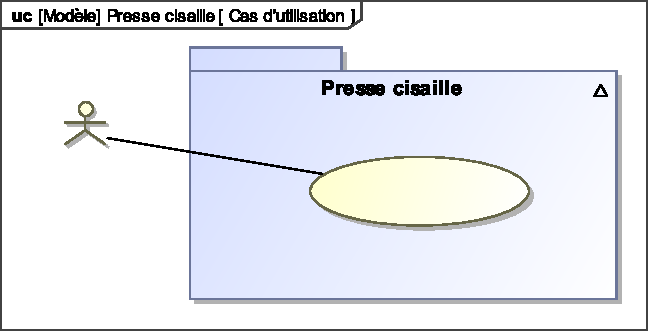
\includegraphics[width=0.8\linewidth]{img/use_case_vierge}
\end{center}

\newpage

\paragraph{Question 3:}

\begin{center}
 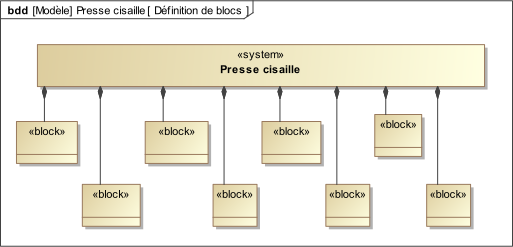
\includegraphics[width=0.8\linewidth]{img/BDD_vierge}
\end{center}

\paragraph{Question 4:}

\begin{center}
 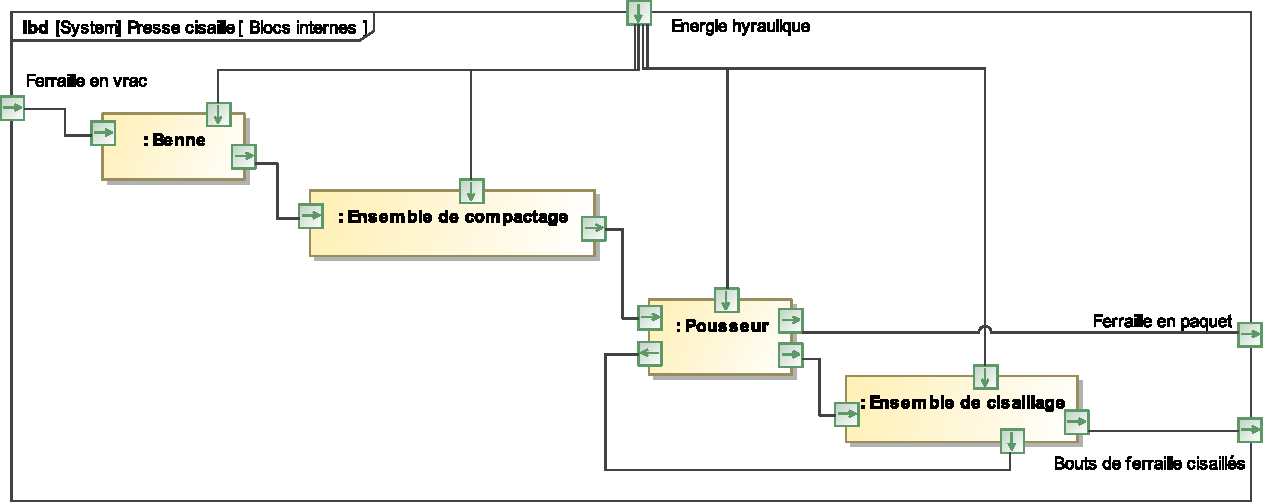
\includegraphics[width=0.8\linewidth]{img/Blocs_internes_vierge}
\end{center}

\newpage
\cleardoublepage

Nom:.....................\\
Prénom:......................

~\

\paragraph{Question 5:}

\reponse[5]

\paragraph{Question 6:}

\reponse[5]


\paragraph{Question 7:}

\reponse[5]

\paragraph{Question 8:}

\reponse[5]

\paragraph{Question 9:}

\reponse[5]

\paragraph{Question 10:}

\reponse[5]

\paragraph{Question 11:}

\reponse[5]


\iffalse
\paragraph{Question 7:}

\begin{center}
 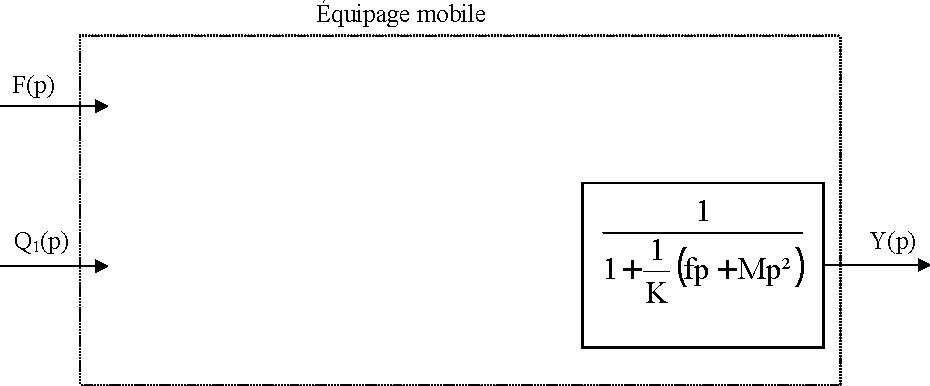
\includegraphics[width=0.8\linewidth]{img/SB1}
\end{center}

\paragraph{Question 9:}

\begin{center}
 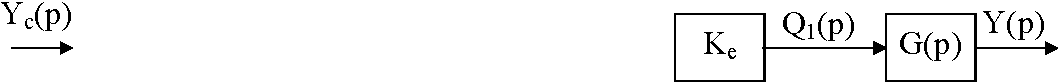
\includegraphics[width=0.8\linewidth]{img/SB2}
\end{center}

\vspace{1cm}
\fi

\paragraph{Question 12:}

\begin{center}
 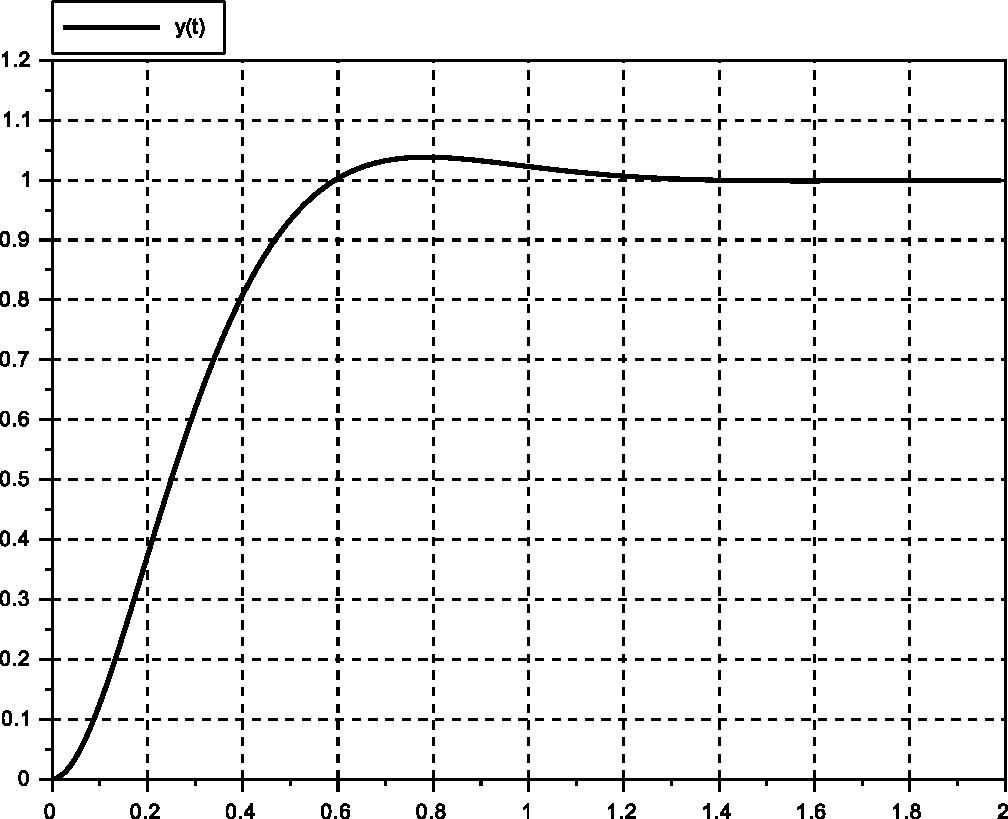
\includegraphics[width=0.7\linewidth]{img/courbe}
\end{center}


~\

\cleardoublepage

Nom:.....................\\
Prénom:......................

\paragraph{Question 13:}

\begin{center}
 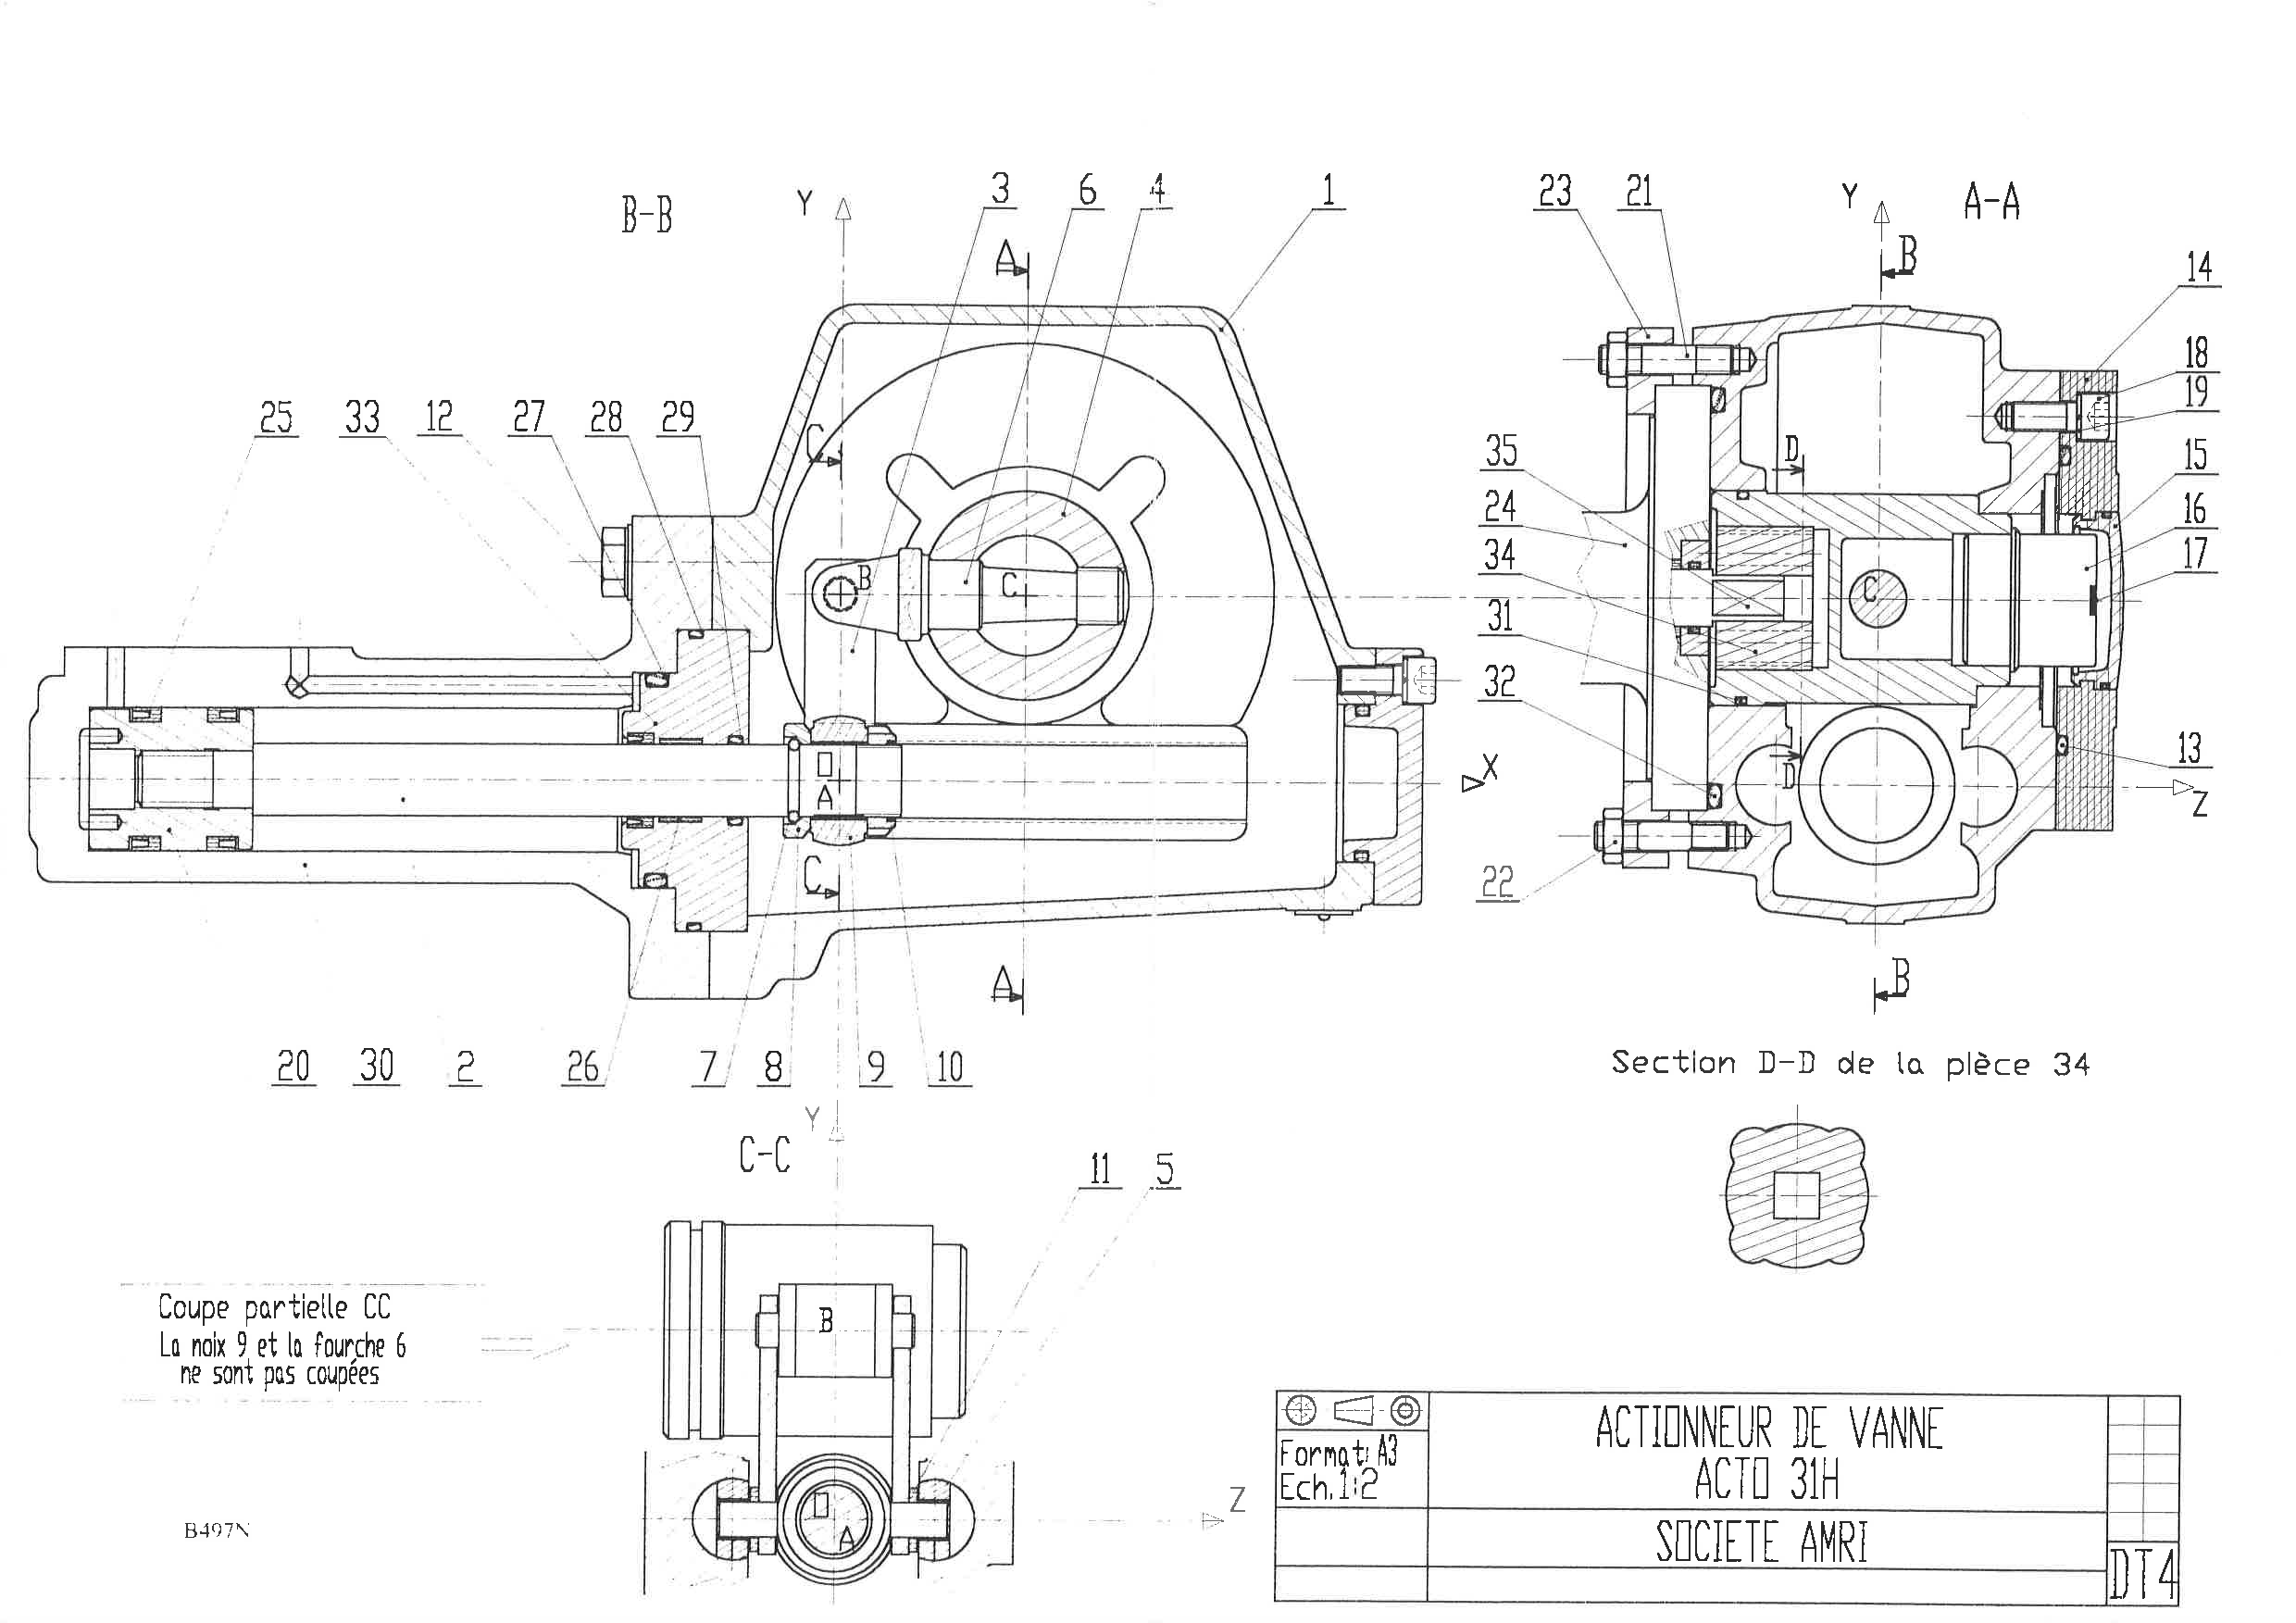
\includegraphics[width=1.3\linewidth,angle=-90]{img/Actionneur_vanne}
\end{center}


\paragraph{Question 14:}

\reponse[7]

\paragraph{Question 15:}

\reponse[7]

\ifdef{\public}{\end{document}}{}

\newpage
\cleardoublepage

\pagestyle{correction}

\section{Correction}

\paragraph{Question 1:}

\begin{center}
 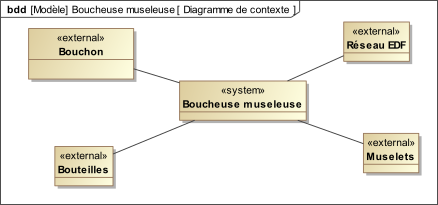
\includegraphics[width=0.8\linewidth]{img/contexte_corrige}
\end{center}

\paragraph{Question 2:}

\begin{center}
 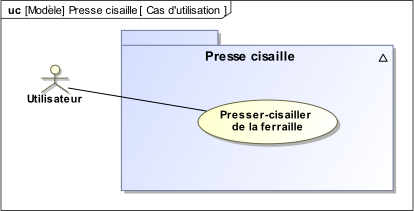
\includegraphics[width=0.8\linewidth]{img/use_case_corrige}
\end{center}

\paragraph{Question 3:}

\begin{center}
 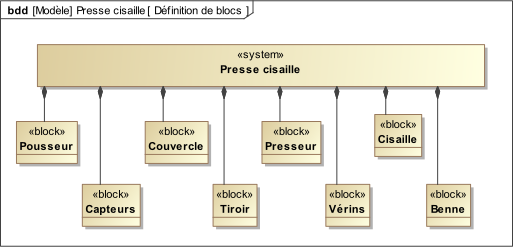
\includegraphics[width=0.8\linewidth]{img/BDD_corrige}
\end{center}

\paragraph{Question 4:}

\begin{center}
 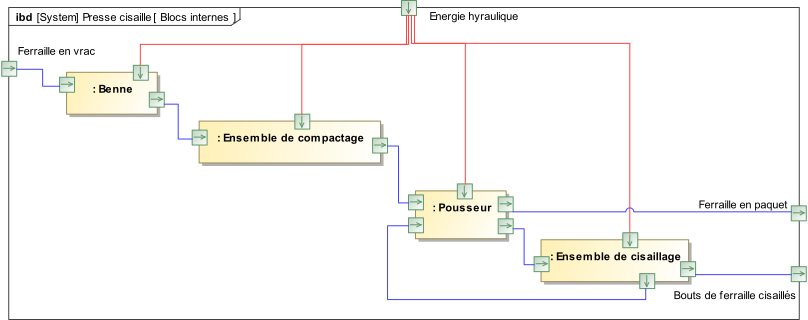
\includegraphics[width=0.8\linewidth]{img/Blocs_internes_corrige}
\end{center}

\paragraph{Question 5:}

$H_1(p)=\dfrac{\dfrac{1}{S_1}}{p.\left(\dfrac{M}{K}.p^2+\dfrac{f}{K}.p+1\right)}$

$H_2(p)=\dfrac{\dfrac{1}{K}}{\left(\dfrac{M}{K}.p^2+\dfrac{f}{K}.p+1\right)}$

\paragraph{Question 6:}

$Y(p)=\dfrac{\dfrac{1}{S_1}}{p.\left(\dfrac{M}{K}.p^2+\dfrac{f}{K}.p+1\right)}.Q_1(p)+\dfrac{\dfrac{1}{K}}{\left(\dfrac{M}{K}.p^2+\dfrac{f}{K}.p+1\right)}.F(p)$

\iffalse
\begin{center}
 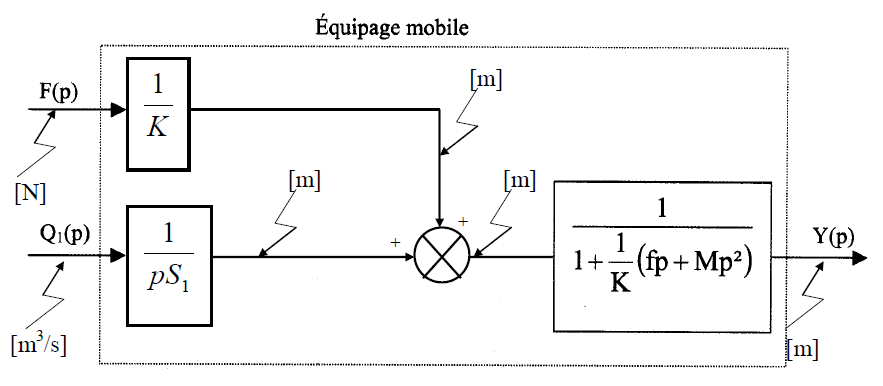
\includegraphics[width=0.8\linewidth]{img/SB1_corrige}
\end{center}
\fi

\paragraph{Question 7:}

$\dfrac{U_s(p)}{Y(p)}=K_c$,
$\dfrac{Q_1(p)}{U_e(p)}=K_e$


\paragraph{Question 8:}

$\dfrac{U_s(p)}{U_e(p)}=\dfrac{U_s(p)}{Y(p)}\times\dfrac{Y(p)}{Q_1(p)}\times\dfrac{Q_1(p)}{U_e(p)}=\dfrac{\dfrac{K_c.K_e}{S_1}}{p.\left(\dfrac{M}{K}.p^2+\dfrac{f}{K}.p+1\right)}$

\paragraph{Question 9:}

Ordre 3, classe 1, $K=\dfrac{K_c.K_e}{S_1}$, $\omega_0=\sqrt{\frac{K}{M}}$, $\xi=\frac{f}{2\sqrt{K.M}}$.

\paragraph{Question 10:}

$\left[K_c.Y_c(p)-U_s(p)\right] \times A=U_e(p)$

$U_s(p)=Kc.Y(p)$

$\dfrac{Y(p)}{U_e(p)}=\dfrac{Y(p)}{Q_1(p)}\times \dfrac{Q_1(p)}{U_e(p)}=\dfrac{K_e}{p.S_1.(1+\frac{1}{K}.(f.p+M.p^2))}$

$\dfrac{Y(p)}{Y_c(p)}=\dfrac{1}{1+\dfrac{S_1}{A.K_c.K_e}.p+\dfrac{f.S_1}{A.K_c.K_e.K}.p^2+\dfrac{M.S_1}{A.K_c.K_e.K}.p^3}$

\paragraph{Question 11:}

Sachant que M est négligeable, la fonction de transfert précédente peut s'écrire:

$\dfrac{Y(p)}{Y_c(p)}=\dfrac{1}{1+\dfrac{S_1}{A.K_c.K_e}.p+\dfrac{f.S_1}{A.K_c.K_e.K}.p^2}$

$\omega_0=\sqrt{\dfrac{A.K_c.K_e.K}{f.S_1}}=5.77rad.s^{-1}$

$\xi=\dfrac{1}{2}.\sqrt{\dfrac{K.S_1}{f.A.K_c.K_e}}=0,72$

\paragraph{Question 12:} 

$D\%=100.e^{-\xi.\dfrac{\pi}{\sqrt{1-\xi^2}}}=3,78\%$

$t_{R,5\%}=\dfrac{1}{\xi.\omega_0}.ln(20)=0,72s$

\begin{center}
 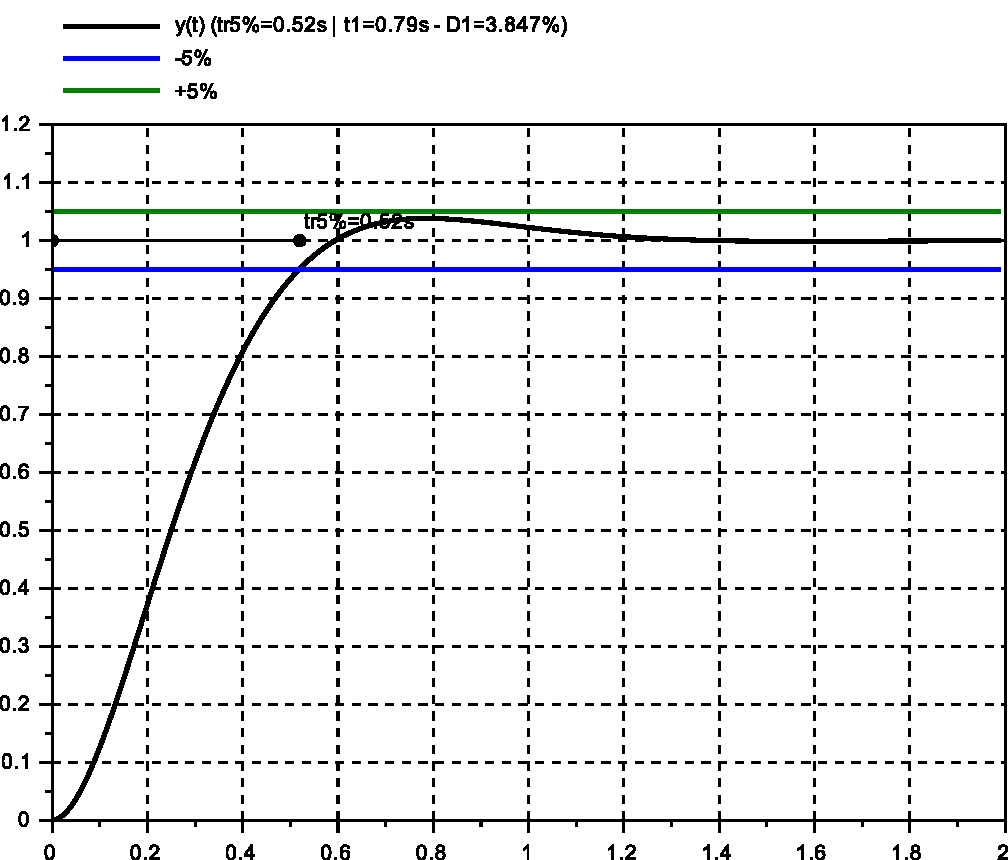
\includegraphics[width=0.8\linewidth]{img/courbe_corrige}
\end{center}

\newpage

\paragraph{Question 13:} 

\begin{center}
 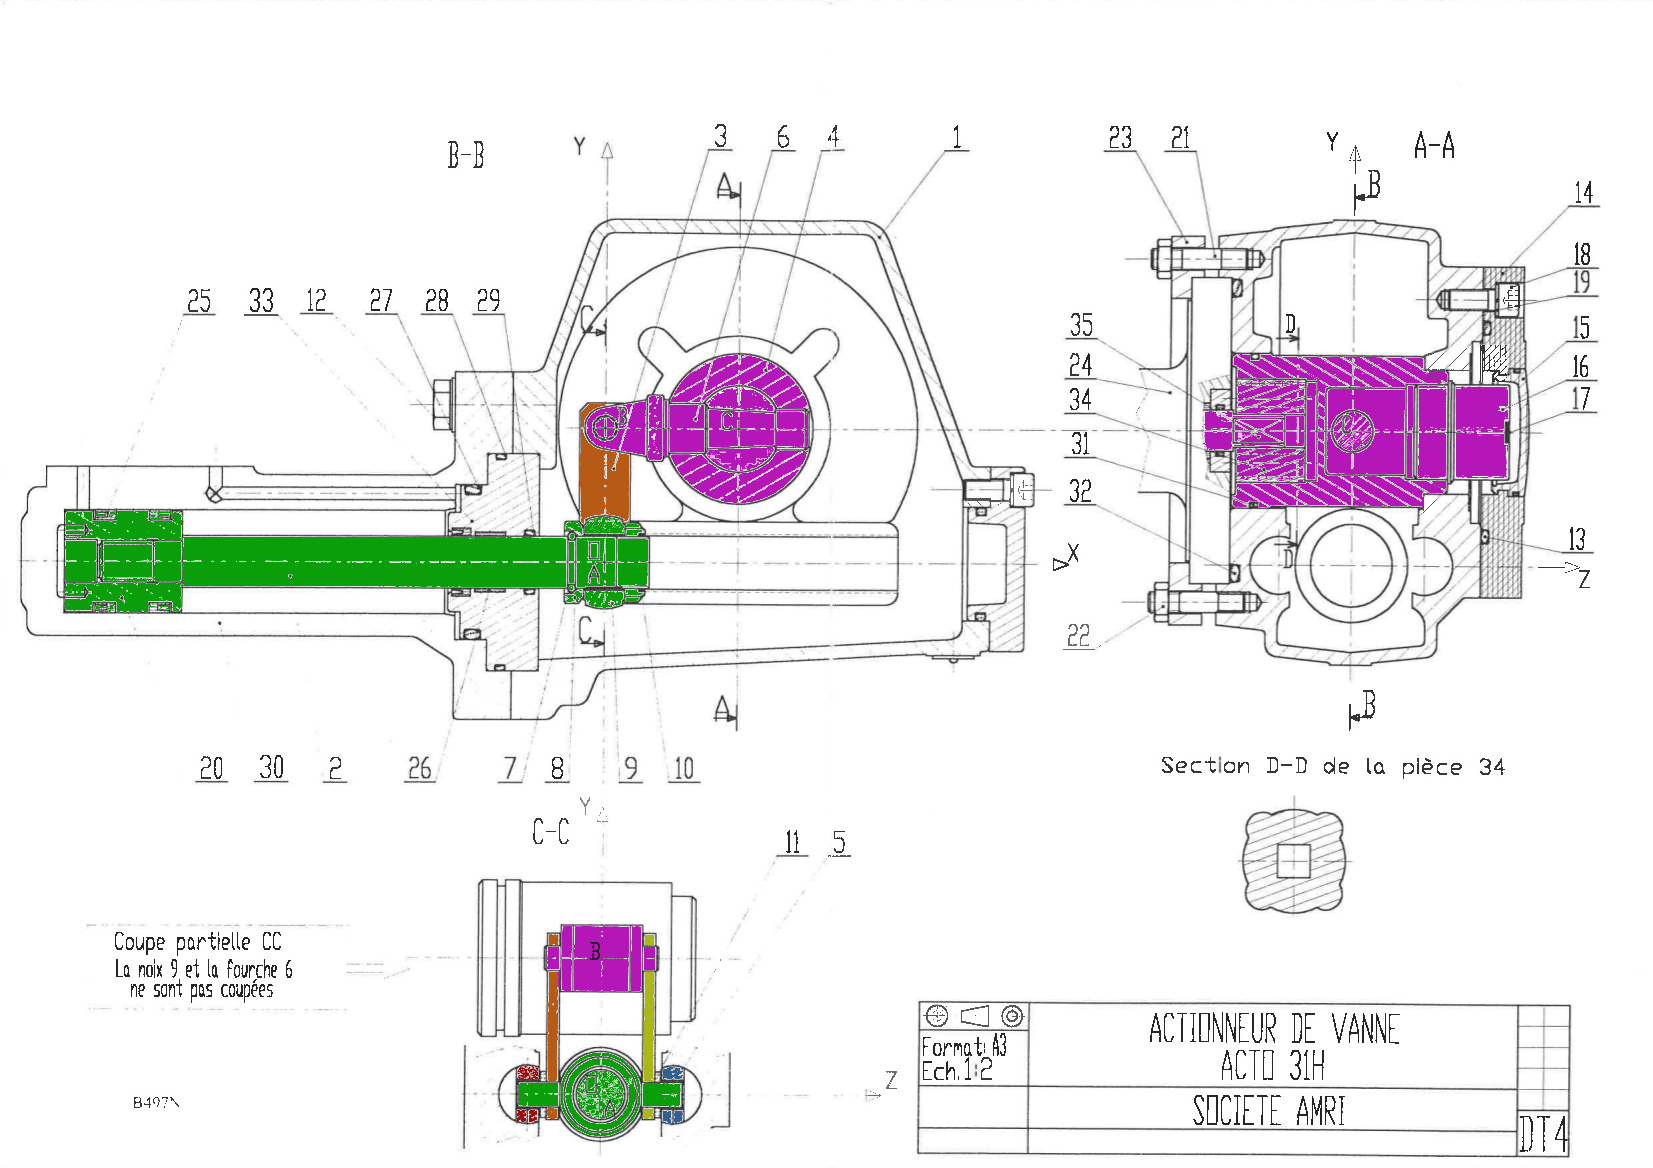
\includegraphics[width=0.8\linewidth]{img/Actionneur_vanne_corrige}
\end{center}

\paragraph{Question 14:} Le mouvement est assuré par un vérin il s'agit donc d'énergie hydraulique (pneumatique peut être acceptée même si elle ne peut pas fournir assez d'efforts).

\paragraph{Question 15:} 

\begin{center}
 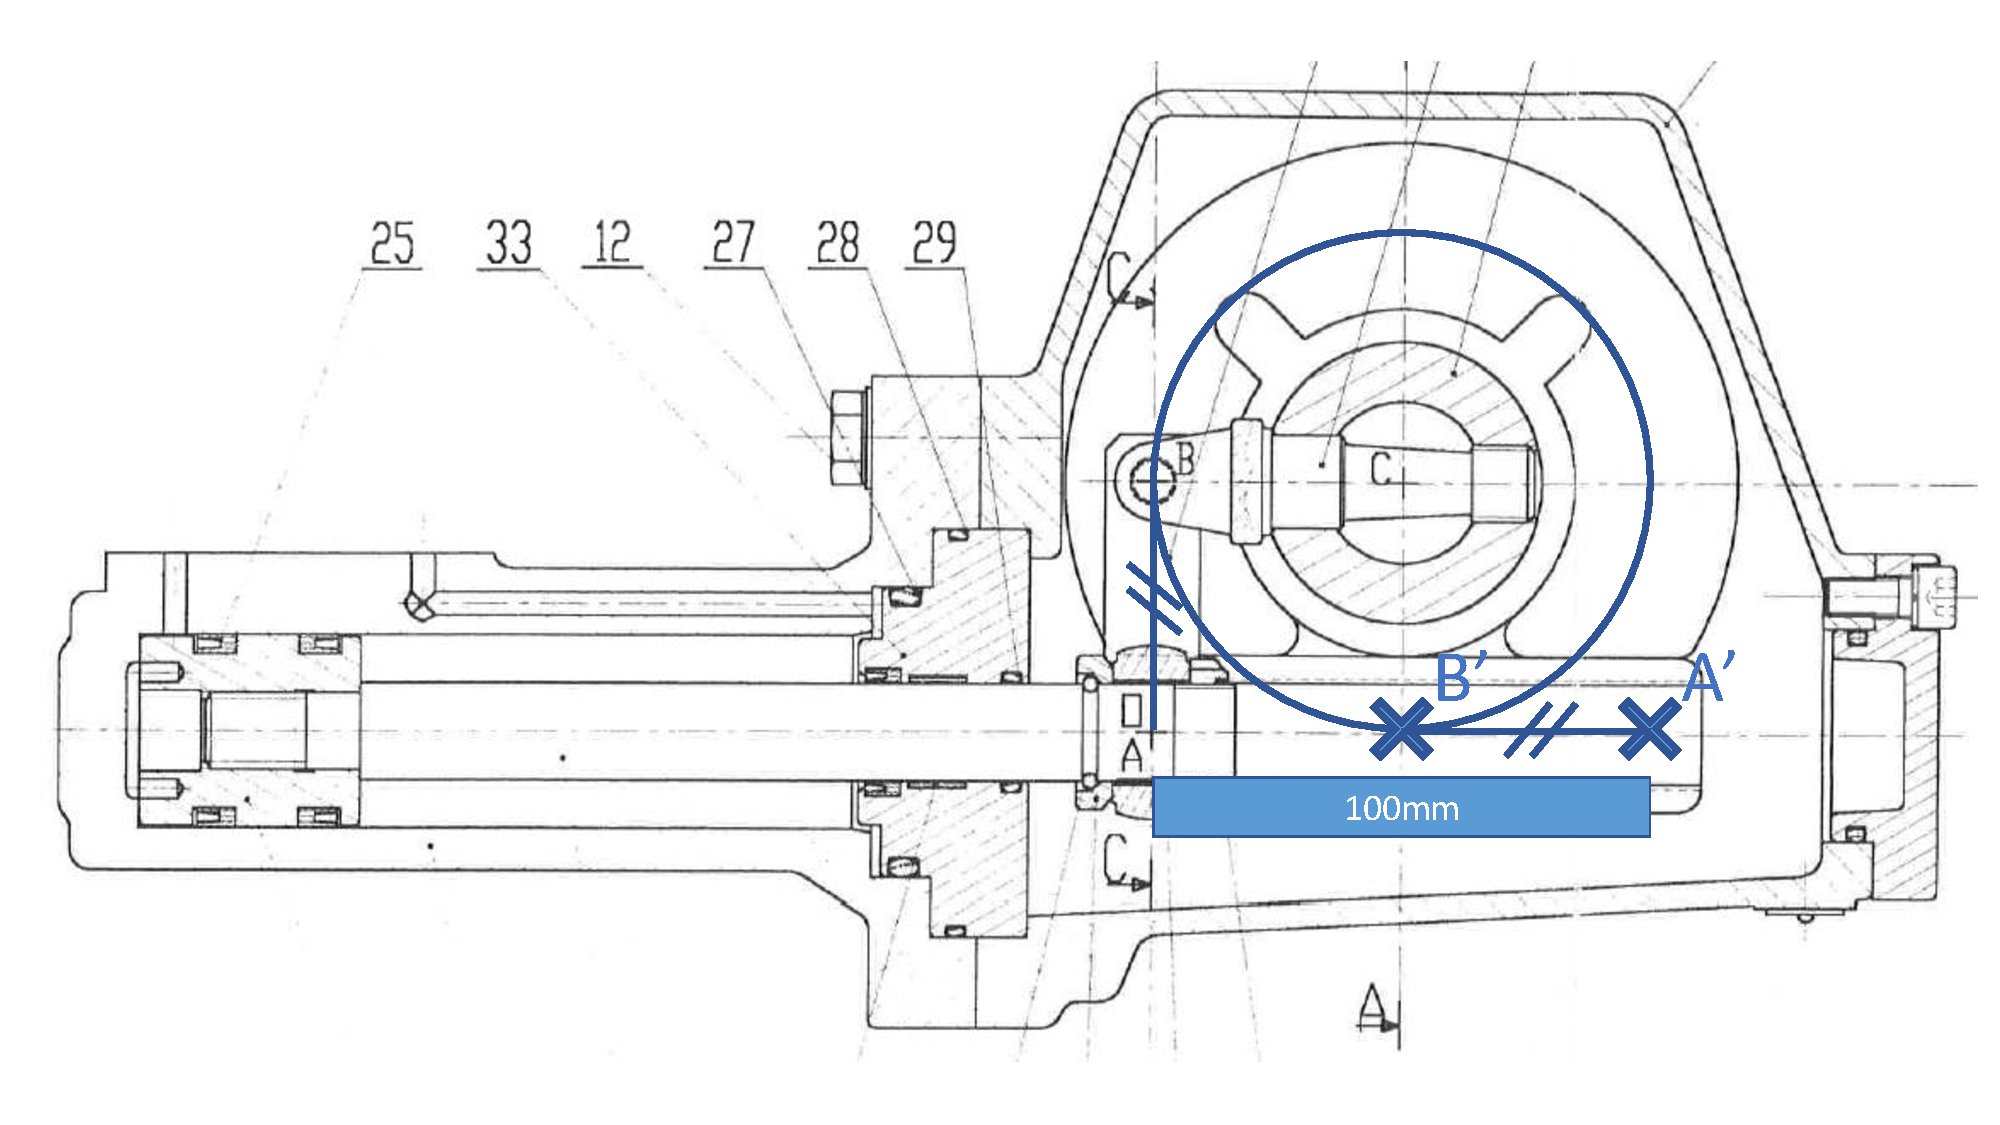
\includegraphics[width=0.8\linewidth]{img/trace_corrige}
\end{center}

Le déplacement est donc de 192mm.

\end{document}

